% !Mode:: "TeX:UTF-8"

\chapter{超像素分割}

\begin{figure*}[h]
\begin{center}
%\fbox{\rule{0pt}{2in} \rule{.9\linewidth}{0pt}}
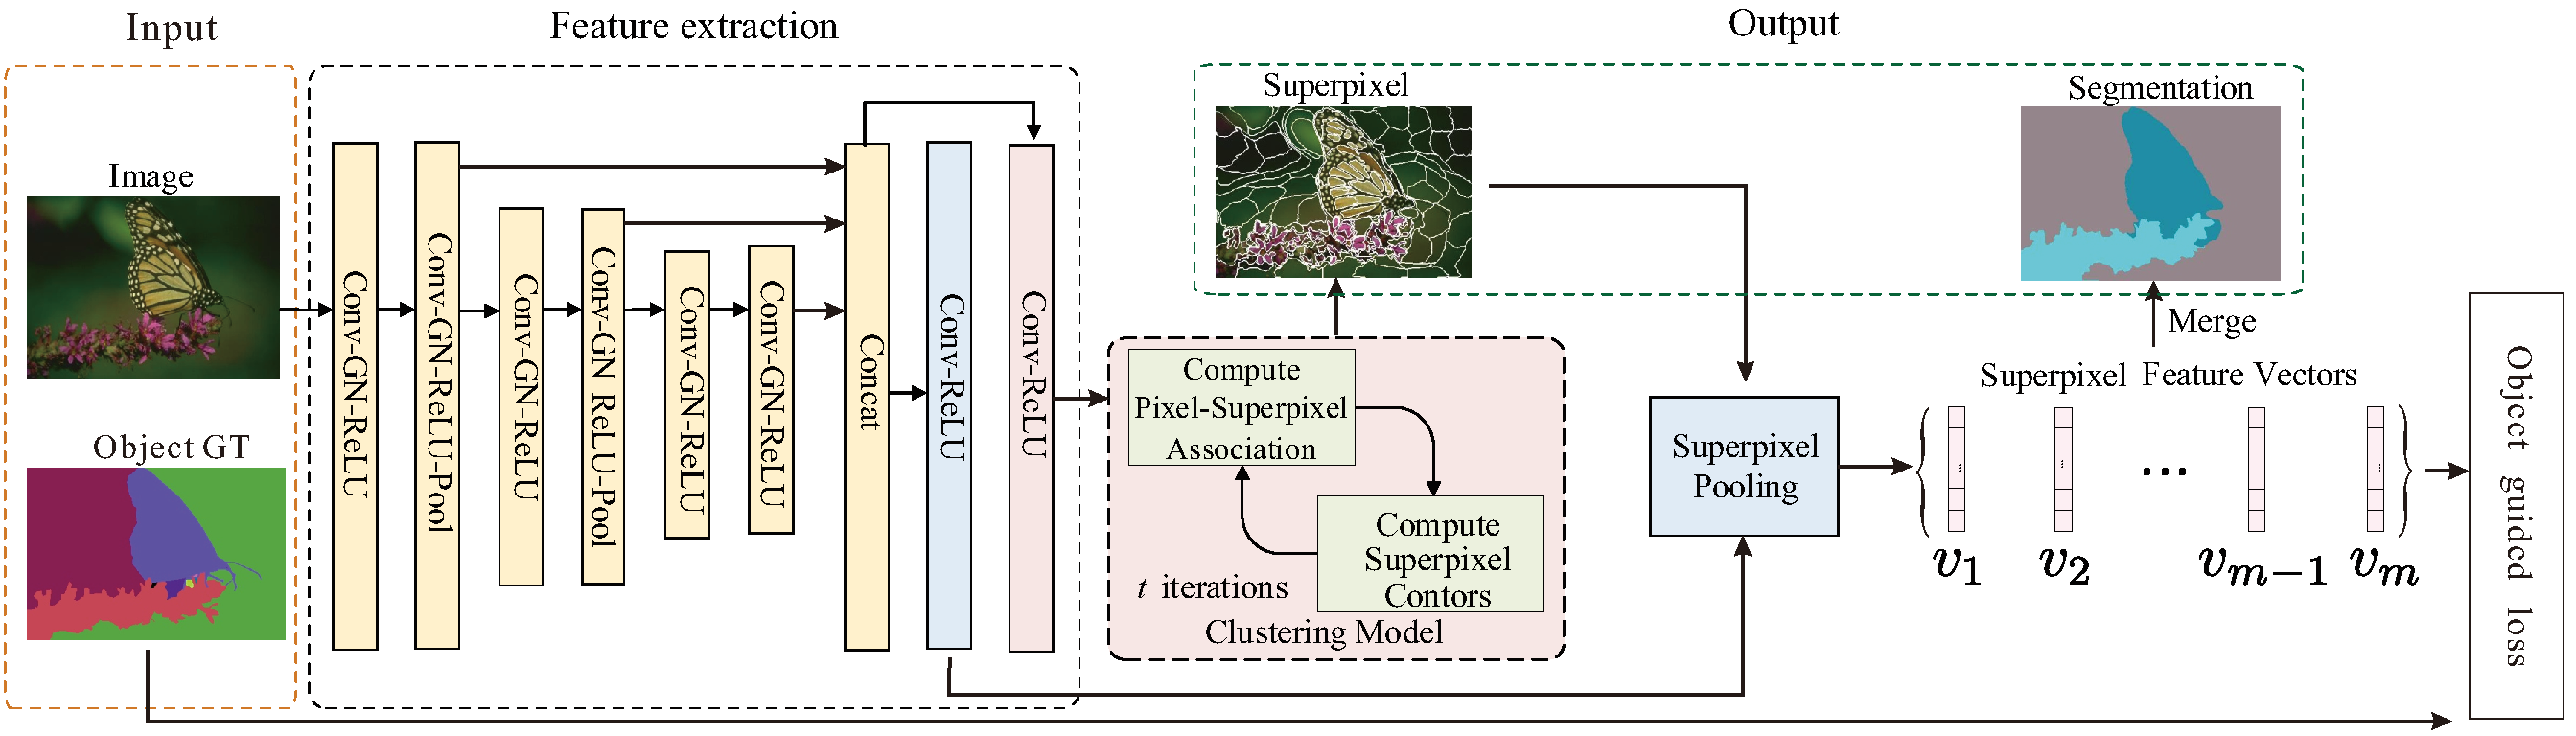
\includegraphics[width=1\textwidth]{figures/img/pipeline.pdf}
\end{center}
\vspace{-5mm}
\caption{算法流程图。对于给定的图像,我们的算法同时生成超像素和图像分割。输入图像首先被输送到一个特征提取网络,该网络由一系列卷积层、归一化(GN)和ReLU操作组成。然后将提取的特征输入可微聚类模块,生成超像素。超像素池用于获取超像素特征向量。最后通过合并相似度高的超像素实现图像分割}
\label{Fig.sub.1}
\end{figure*}

如图3-1所示,我们的方法首先从CNN深度网络中学习图像特征,然后我们使用迭代可微分聚类算法模块来获取超像素。接下来,我们通过超像素池化层计算超像素特征向量,并计算相邻超像素之间的相似性。最后,根据相似度判断相邻的两个超像素是否合并。在本节中,我们将详细介绍我们的方法。

\section{超像素生成}

超像素将相似像素分组为各向同性区域,从而可以提高分割质量和效率。 例如,在DEL算法中,作者使用SLIC作为图像分割的开始。在本文中,与采用现有的超像素算法进行图像分割的方法不同,我们将超像素生成作为图像分割网络的一部分。为此,我们采用SSN中提出的可微聚类算法模块,以取代SLIC算法中的硬像素-超像素关联。

\subsection{SLIC中的硬链接}
通常,对于$n$像素的图像\(I\in\mathbb{R}^{n\times 5}\),在CIELAB空间的特征为$I_p=[x,y,l,a,b]$ ,我们希望将其划分为$m$ 个小区域,即将图片分成m个超像素。在介绍在描述软关联之前,我们简要介绍SLIC算法中如何计算像素-超像素硬关联$H = \left \{1, 2, \cdots, m \right \}^{n\times 1}$。给定统一采样的超像素中心$C^{0}$作为初始值,SLIC算法在每次迭代$t$中计算每个像素$p$处的新超像素分配,
\begin{equation}\label{eqn:hardassn}
H_{p}^{t} =  \mathop{{{\rm argmin}}}\limits_{{i\in\{ 1, 2, \cdots ,m \} }}\left\|I_{p}-C_{i}^{t-1}\right\|_2,
\end{equation}
其中$\|\cdot\|_2$表示输入向量的$\ell_2$范数,$C_i^{t-1}$表示超像素中心$i$的特征,该特征通过对第$t$次迭代后,计算属于该超像素中心的像素的特征平均值来获取。

\subsection{本文的方法}

由于(3-1)获取像素-超像素硬关联H的操作是不可微的,因此SLIC无法直接集成到神经网络中。 在我们算法中的用到的可微分聚类算法模块,其将硬像素-超像素硬关联H替换为软关联Q。与原始SLIC相似,它在每次迭代中具有以下两个核心步骤:

1.	像素-超像素关联计算。第t次迭代中像素p及其相邻超像素i之间的关联计算如下:
\begin{equation}
Q_{pi}^{t} = e^{-\left \| F_{p}-C_{i}^{t-1}\right \|_2^2},
\end{equation}
其中\(F_{p}\)是像素$p$的深层特征。 在我们的情况下,它来自我们网络的特征提取模块。\(Q_{pi}^{t}\)是$t$次迭代后像素$p$与超像素中心$i$之间的距离。

2.	超像素中心更新。新的超像素聚类中心是根据像素特征的加权总和得出的,
\begin{equation}
C_{i}^{t} = \frac{1}{Z_{i}^{t}}\sum_{p}Q_{pi}^{t}F_{p},
\end{equation}
其中$Z_{i}^{t}$表示归一化过程,即$Z_{i}^{t} = \sum\nolimits_{p}Q_{pi}^{t} $ 。

将这两个步骤迭代数次(在本文中,设定迭代次数为10次),最终得到像素-超像素软关联\(Q\in\mathbb{R}^{n\times m}\)。与(3-1)相似,我们需要计算硬关联映射$H'\in \mathbb{R}^{n\times 1}$,最终得到像素$p$的超像素标签,
\begin{equation}
H'_{p} =  \mathop{{{\rm argmax}}}\limits_{{i \in \left\{ 1, \cdots ,m \right\} }}Q_{pi}.
\label{equation.3}
\end{equation}

值得注意的是,这种硬关联的计算是不可微的。因此在我们的算法中,这一步不参与反向传播。在实验中,我们发现计算像素和超像素聚类中心之间的软关联非常耗时。与SLIC相似,我们只是计算每个像素到周围超像素聚类中心的距离,大大减少了计算时间。

\section{损失函数}

\subsection{像素和超像素表示之间的映射}

利用提供硬聚类的传统超像素算法,这种从像素到超像素表示的映射是通过在每个聚类内部进行平均来完成的。从超像素到像素表示的逆映射是通过将相同的超像素特征分配给属于该超像素的所有像素来完成的。
然而,由于这种硬关联的计算是不可微的,因此在集成到端到端可训练系统时可能不希望使用硬簇。
值得注意的是,由网络生成的像素 - 超像素软连接也可以容易地用于像素和超像素表示之间的映射。方程4已经描述了从像素到超像素表示的映射,其是与列标准化Q矩阵的转置的简单矩阵乘法:$S=\hat{Q}^{T}F$,其中F和S分别表示像素和超像素。从超像素到像素表示的逆映射是通过将行标准化Q(表示为$\tilde{Q}$)。与超像素表示($F = \tilde{Q}S$)相乘。因此,像素 - 超像素特征映射被给出为具有关联矩阵的简单矩阵乘法并且是不可分的。之后,我们将利用这些映射来设计损失函数。

\subsection{重建损失}

本文把像素属性表示为$R\in \mathbb{R}^{n\times l}$。
如前所述,我们可以使用列标准化关联矩阵$\hat{Q}$,$\breve{R}=\hat{Q}^{T}R$将像素属性映射到超像素上,
其中$\breve{R}\in \mathbb{R}^{m\times l}$。
然后使用行标准化关联矩阵$\tilde{Q}$ ,将得到的超像素表示$\breve{R}$映射回像素表示$R^{\ast }$,
$R^{\ast } = \tilde{Q}S$ 其中$R^{\ast } \in \mathbb{R}^{n\times l}$。
然后重建损失给出为:

\begin{equation}
L = \mathscr{L}(R,R^{*}) = \mathscr{L}(R,\tilde{Q}\hat{Q}^{T}R)
\end{equation}

本文使用$\ell_1$交叉熵损失来学习的超像素。这里Q表示在可微聚类模块的最终迭代之后的关联矩阵$Q^{v}$。
为方便起见,我们省略了$v$。

\subsection{紧凑性损失}

除了上述损失之外,本文还使用紧凑性损失来鼓励超像素在空间上紧凑,即在每个超像素簇内具有较低的空间变化。让$I^xy$表示位置像素特征。我们首先将这些位置特征映射到我们的超像素表示中,$S^xy=\hat{Q}^{T}I^{xy}$。然后,通过将相同的超像素位置特征分配给属于该超像素的所有像素,$\bar{I}_{p}^{xy} = S_{i}^{xy}\mid H_{p}=i$,使用硬关联H而不是软关联Q对像素表示进行逆映射。紧凑性损失定义为以下$\ell_2$规范:
\begin{equation}
L = \left \|I^{xy}-\bar{I}^{xy} \right \|_{2}
\end{equation}

这种损失促使超像素具有较低的空间方差。